\documentclass{article}

\usepackage{graphicx}
\usepackage[utf8]{inputenc}
\usepackage[english]{babel}

\usepackage{algorithm}
\usepackage[noend]{algpseudocode}

\usepackage{afterpage}

\usepackage{subcaption}
\usepackage{array}
\newcolumntype{P}[1]{>{\centering\arraybackslash}p{#1}}
\usepackage{booktabs,makecell}
\usepackage{color} 


\setlength{\parindent}{1em}
\setlength{\parskip}{1.5em}
\renewcommand{\baselinestretch}{1.2}



\usepackage{geometry}
\geometry{a4paper , portrait, margin=1.3in}



\newcommand*{\eg}{e.g.\@\xspace}
\newcommand*{\ie}{i.e.\@\xspace}
\newcommand*{\etal}{\textit{et~al.}\@\xspace}

\makeatletter
\def\hlinewd#1{%
	\noalign{\ifnum0=`}\fi\hrule \@height #1 %
	\futurelet\reserved@a\@xhline}
\makeatother 

\title{ \textbf{Learning the basics commands of \\ Command Prompt}}
\author{Cyprus University of Techology \\ \\ Milto Miltiadou}
\date{March 8th, 2017}

\begin{document}
	\setlength{\parindent}{0cm}
		\maketitle
			\setcounter{secnumdepth}{0}
		\section{Introduction}
		
	\par This tutorial gives you an overview of the basic line commands that can be executed using the Microsoft Windows  Command Prompt available on windows machines. By following the procedures of this tutorial, you will learn to: 
	
	\begin{enumerate}
		\item Open Command Prompt on Windows
		\item View the contents of a directory 
		\item Change directory
		\item More useful commands
		\item Executing multiple commands using .bat files 
	\end{enumerate}
			\setcounter{secnumdepth}{3}
			
	\section{Opening the Command Prompt window}
	 
	 \par The Command Prompt is the command-line interpreter on Windows machines. For example, it allows you to execute line commands for opening or modifying files. For windows 7 and lower, the Command Prompt is found by searching "Command Prompt" on the Star Menu Search bar (Figure \ref{fig:Windows7}). For windows 10, you will find it by pressing right click on the start icon (Figure \ref{fig:Windows10}). Inside the black window that appears, we can write and execute  commands. Figure \ref{fig:CommandPrompt} shows a Command Prompt window. The follow sections give an overview of a few basic commands. 
	 
	 \afterpage{
	 	 	\begin{figure} [h!]	 		
	 	 	
	 	 		\begin{subfigure}[t]{.49\textwidth}
	 	 			\centering
	 	 			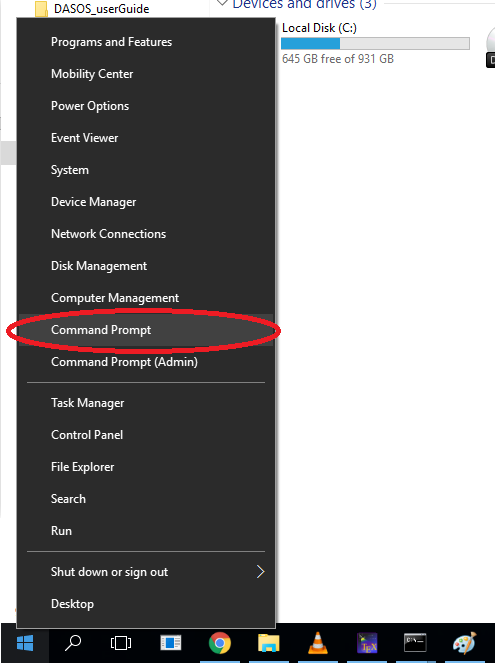
\includegraphics[width=.9\textwidth]{findCommandPrompt.png}
	 	 			\caption{Open Command Prompt on Windows 7 and older versions.} 
	 	 			\label{fig:Windows7}
	 	 		\end{subfigure} \hfill 
 	 			\begin{subfigure}[t]{.49\textwidth}		
	 	 			\centering
	 	 			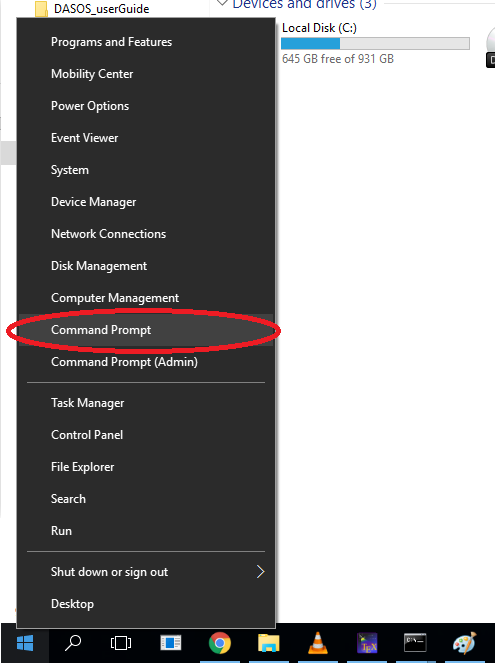
\includegraphics[width=.9\textwidth]{findCommandPrompt.png}
	 	 			\caption{Open Command Prompt on Windows 10.}
	 	 			\label{fig:Windows10}
		 	 	 \end{subfigure} \hfill	 	 			
	 	 		\caption{How to open the Command Prompt.}
	 	 		\label{fig:OpenCommandPrompt} 
	 	 	\end{figure}
	 	 	
	 	 	\begin{figure}[!htbp]
	 	 		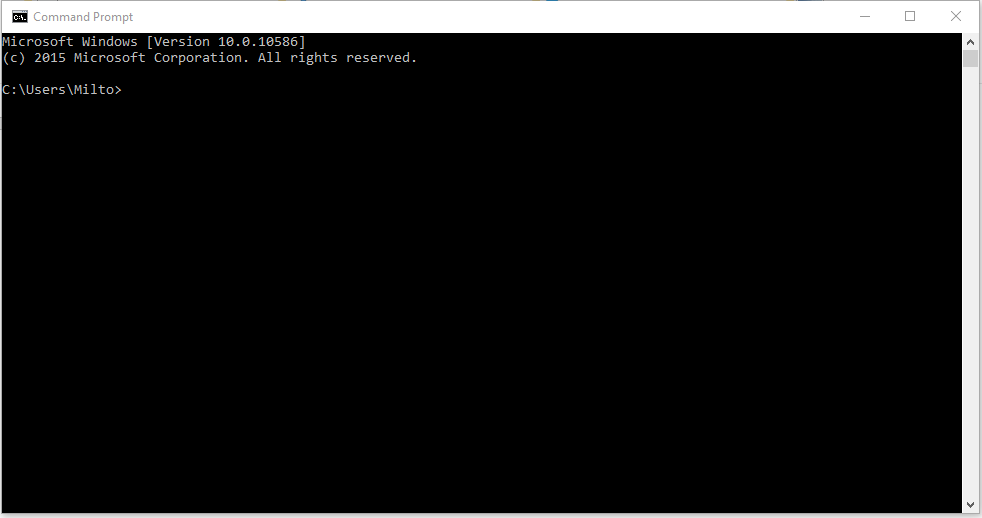
\includegraphics[width=\textwidth]{CommandPrompt.png}
	 	 		\caption{The Command Prompt Window}
	 	 		\label{fig:CommandPrompt}
	 	 	\end{figure}
	 	 }
	
	\newpage \newpage
	\section{Viewing the contents of a directory  - $<$dir$>$}
	\par In order to view the content of the current directory we use the command \textbf{dir}. The name of the command \textbf{dir} is derived from the word "directory".  
	
	\par Type the following at the command prompt and press enter:
	
	\par \$: \textbf{dir}
	 
	\par A list similar to the following appears:
	

		\setlength{\parindent}{-0.125cm}
\par \textbf{
	24/02/2017 \quad 11:17 \quad  $<$DIR$>$  \quad  \qquad \quad .\newline
	24/02/2017 \quad 11:17 \quad  $<$DIR$>$  \quad  \qquad \quad ..\newline
	28/07/2016 \quad 21:45 \quad  $<$DIR$>$  \quad  \qquad \quad .cache\newline
	01/03/2017 \quad 11:42 \quad  $<$DIR$>$  \quad  \qquad \quad .qgis2\newline
	01/12/2016 \quad 13:09 \quad  \qquad  \qquad   2,032 \quad .recently-used.xbel\newline
	02/03/2017 \quad 11:13 \quad  $<$DIR$>$  \quad  \qquad \quad Desktop\newline
	27/02/2017 \quad 16:58 \quad  $<$DIR$>$  \quad  \qquad \quad Documents\newline
	01/03/2017 \quad15:44  \quad  $<$DIR$>$  \quad  \qquad \quad Downloads\newline
	15/11/2016 \quad 01:44 \quad  $<$DIR$>$  \quad  \qquad \quad Links\newline
	15/11/2016 \quad 01:44 \quad  $<$DIR$>$  \quad  \qquad \quad Music\newline
	02/03/2017 \quad 15:26 \quad  $<$DIR$>$  \quad  \qquad \quad Videos\newline
	}

	\setlength{\parindent}{0cm}
	
	\par This is the list of all the files and subfiles of the working directory, which is the current directory. The working directory is indicated within Command Prompt. As shown Figure \ref{fig:CommandPrompt} the working directory is \textbf{C:\textbackslash Users\textbackslash Milto } and the above list contains all the files and subdirectories of that directory.
	
	\par The  $<$DIR$>$ label indicates that the listed item is a directory itself. If the working directory is not a drive (e.g. \textbf{C:\textbackslash}), the first two directories (\textbf{.} and \textbf{..}) are always listed. The \textbf{.} directory is the current working directory (\textbf{C:\textbackslash Users\textbackslash Milto}) and the \textbf{..} directory is the directory of the folder that contains the working directory (\textbf{C:\textbackslash Users}).
	
	\par When a directory contains many items, the tag \textbf{/p} is very useful. For example, type the following command:
	\par\$:\textbf{ dir /p }
	
	\par This will print a page of the directory list and the next page appears once the button \textbf{Enter} is pressed. 
	
		
	\section{Changing directory - $<$cd$>$}
	\par Moving from one directory to another is essential and the command \textbf{cd} (named after "change directory") is responsible for that. From the working directory (\textbf{C:\textbackslash Users\textbackslash Milto}), you can move to the subdirectory \textbf{Documents} by typing the following: 
	\par \$: \textbf{cd Documents}  
	
	\par Or you may include the entire path of the directory of interest. For example:
	
	\par \$: \textbf{cd C:\textbackslash Users\textbackslash Milto\textbackslash Documents}  
	
	
	\par By the way, when typing a directory you may use the \textbf{tab} button to quickly fill the name's of directories and files. Try typing:
	
	\par \$: \textbf{cd C:\textbackslash Us}
	
	\par and then press tab. It will automatically fill it to \textbf{cd C:\textbackslash Users}. If more than one options apply, we may looping through them by pressing the button \textbf{tab} multiple times. 
	
	\par Additionally, it is essential to be able to move from a working directory to the folder containing that working directory. This is done by the following command:
	
	\par \$: \textbf{cd ..}
	
	\par As mentioned before, the directory \textbf{..} is the directory of the folder that contains the working directory. Therefore, by using the command \textbf{cd} following with \textbf{..} , we can move backwards one folder. 
	
	\par Similarly, the following command does nothing because it brings you to the current directory, which is the \textbf{.} :
	\par \$: \textbf{cd .}
	
	\par The final command related to changing directory for this tutorial is the following: 
	
	\par \$: \textbf{cd \textbackslash}
		
		\par Type the above command in Command Prompt. This command brings you to the root directory, which should by \textbf{C:\textbackslash}. Therefore the Command Prompt should now show:
		\par \textbf{C:\textbackslash $>$}
		\par Please note that for the final command a baskshlash (\textbackslash) is used and not a forward slash (/);
	

	\section{Quick Overview of some useful commands}\label{sec:Commands}
	
	\par There are numerous commands that can be executed from Command Prompt. Here a number of them are listed.
	
	\par To create a directory, use the command \textbf{md} (make directory) as follow. Please replace the $<$directoryName$>$ with the name of the new directory to be created. 
	
	\par \$:\textbf{ md $<$directoryName$>$}
	
	With the command \textbf{rd} (remove directory), an empty directory can be deleted:
	
	\par \$: \textbf{rd $<$directoryName$>$}
	
	For non-empty dirctories the tag \textbackslash s should be added at the end as follow:
	
	\par \$: \textbf{rd $<$directoryName$>$ \textbackslash s} 
	
	\par For renaming a file:
	
	\$: \textbf{ren $<$oldName$>$ $<$newName$>$}
	
	\par For deleting a file:
	
	\$: \textbf{del $<$filename$>$}
	
	\par For copying a file:
	
	\par \$: \textbf{copy $<$file$>$ $<$destination$>$}
	
	\par For example, the following command will copy the \textbf{file.txt} from the directory \textbf{C:Users} inside the folder \textbf{C:\textbackslash HelloWords}:
	
	\par \$: 	\textbf{copy\space\space c:\textbackslash Users\textbackslash file.txt \space c:\textbackslash HelloWorld 
	 }
	 
    \par Similarly the command for moving a file is the following:
    
    
    \par \$: \textbf{move $<$file$>$ $<$destination$>$}
    
    \par The parameter \textbf{NUL} represents te empty/null. Here, there is a hack for quickly generating an empty text file using the copy command: 
    \par \$: \textbf{copy NUL emptyFile.txt }
    
  
	
	\newpage
	\section{Executing multiple commands using batch (.bat) files}
	\par A batch file is a script file in Microsoft Windows. It consists of a series of commands, which are stored in a plain text file (most commonly with extension .bat). These commands can be executed by the command-line interpreter (Command Prompt).
    
    \par Figure \ref{fig:BatchFile} shows an example of a batch file that uses commands explained in this tutorial. Each line that starts with \textbf{::} is a comment, which means that they are ignored at execution time and they do not influence the interpretation of the commands. 
	
		\begin{figure}[!htbp]
			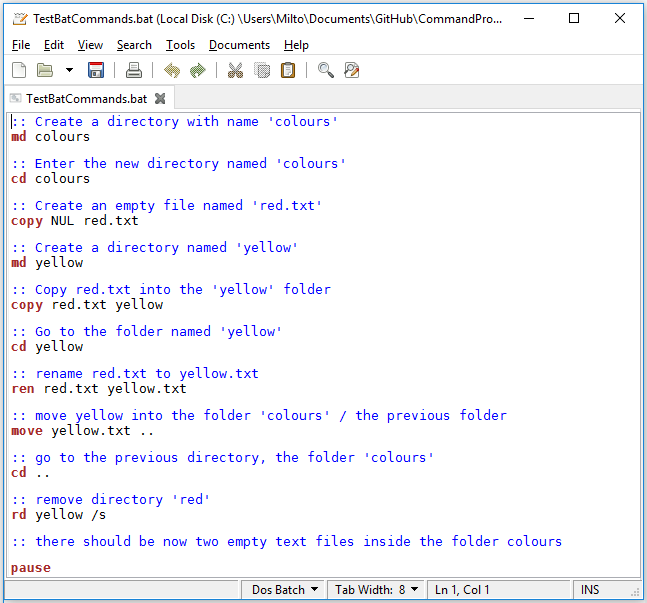
\includegraphics[width=\textwidth]{BatCommands.png}
			\caption{The Command Prompt Window}
			\label{fig:BatchFile}
		\end{figure}
	 
	\par As mentioned before, batch files are plain text files and they can therefore been edited using a text editor. A good option for editing batch files is the gedit application, which also colours the commands. If gedit is not available, then WordPad will also work fine, but preferably avoid using notepad because notepad fails to identify new lines and editing with it is confusing. 
	
	\par To run a batch script file, just double click on the file and all the commands will be executed. 
	
%	\section{Conclusions}
%	This is a tutorial for the basics of the Windows command-line interpreter. In this tutorial, we learned how to open the command prompt, execute simple commands and write batch scripts. 
\end{document}

